\chapter{Gradle}
\section{Поиск отсутствующих зависимосте}
При попытке собрать проект, командой: \texttt{./gradlew~build},
в файле ClientController был обнаружен импорт на не зарегистрированную
зависимость \texttt{import~com.opencsv.bean.CsvToBeanBuilder}.
Сообщение об ошибке показано на рисунке~\ref{fig:gradle:dep:undisc:error}.

\begin{image}
	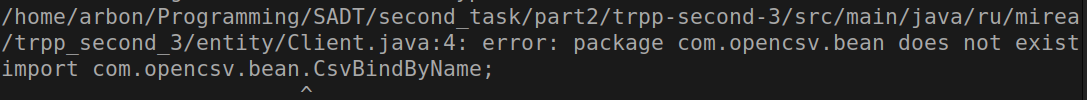
\includegraphics[width=0.8\textwidth]{Screenshot from 2023-03-12 18-05-52.png}
	\caption{Ошибка зависимоти}
	\label{fig:gradle:dep:undisc:error}
\end{image}

Поэтому файл build.gradle была изменен как показано
на рисунке~\ref{fig:gradle:dep:undisc:good}.

\begin{figure}[h!tp]
	\centering
	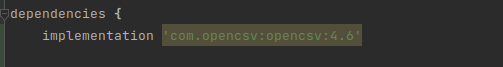
\includegraphics[width=0.8\textwidth]{Screenshot from 2023-03-12 17-25-18.png}
	\caption{Устраниение ошибки зависимости}
	\label{fig:gradle:dep:undisc:good}
\end{figure}

\section{Правка имени пакета}
При попытке собрать проект, командой: \texttt{./gradlew~build},
в файле ClientController были обнаружены не импортируемые пакеты.
Сообщение об ошибке показано на рисунке~\ref{fig:gradle:imp:error}.
Поэтому в соответствующие файлы были внесены необходимые строки.

\begin{figure}[h!tp]
	\centering
	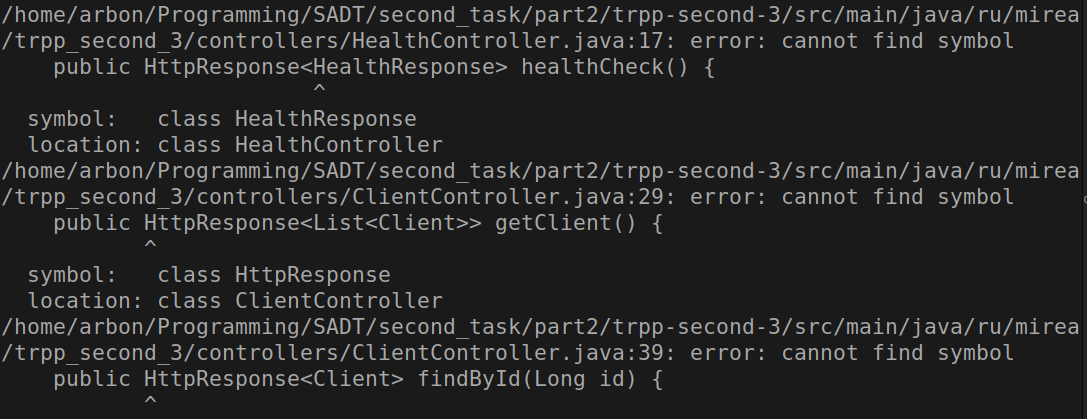
\includegraphics[width=0.8\textwidth]{Screenshot from 2023-03-12 18-16-05.png}
	\caption{Ошибки не омпортируемых пакетов}
	\label{fig:gradle:imp:error}
\end{figure}

А также необходимо исправить имя пакета в файле build.gradle, как показано
на рисунке~\ref{fig:gradle:build:pack}.

\begin{figure}[h!tp]
	\centering
	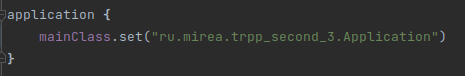
\includegraphics[width=0.8\textwidth]{Screenshot from 2023-03-12 19-08-52.png}
	\caption{Исправление пакет в build.grable}
	\label{fig:gradle:build:pack}
\end{figure}
\section{Сборка документации проект}
Для создания документации использовалась команда: \texttt{./gradlew~javadoc}.
Сгенерированая документация появиться в каталоге gradle/docs.
Пример сгенерированной документации показан
на рисунке~\ref{fig:gradle:javadoc}.

\begin{figure}[h!tp]
	\centering
	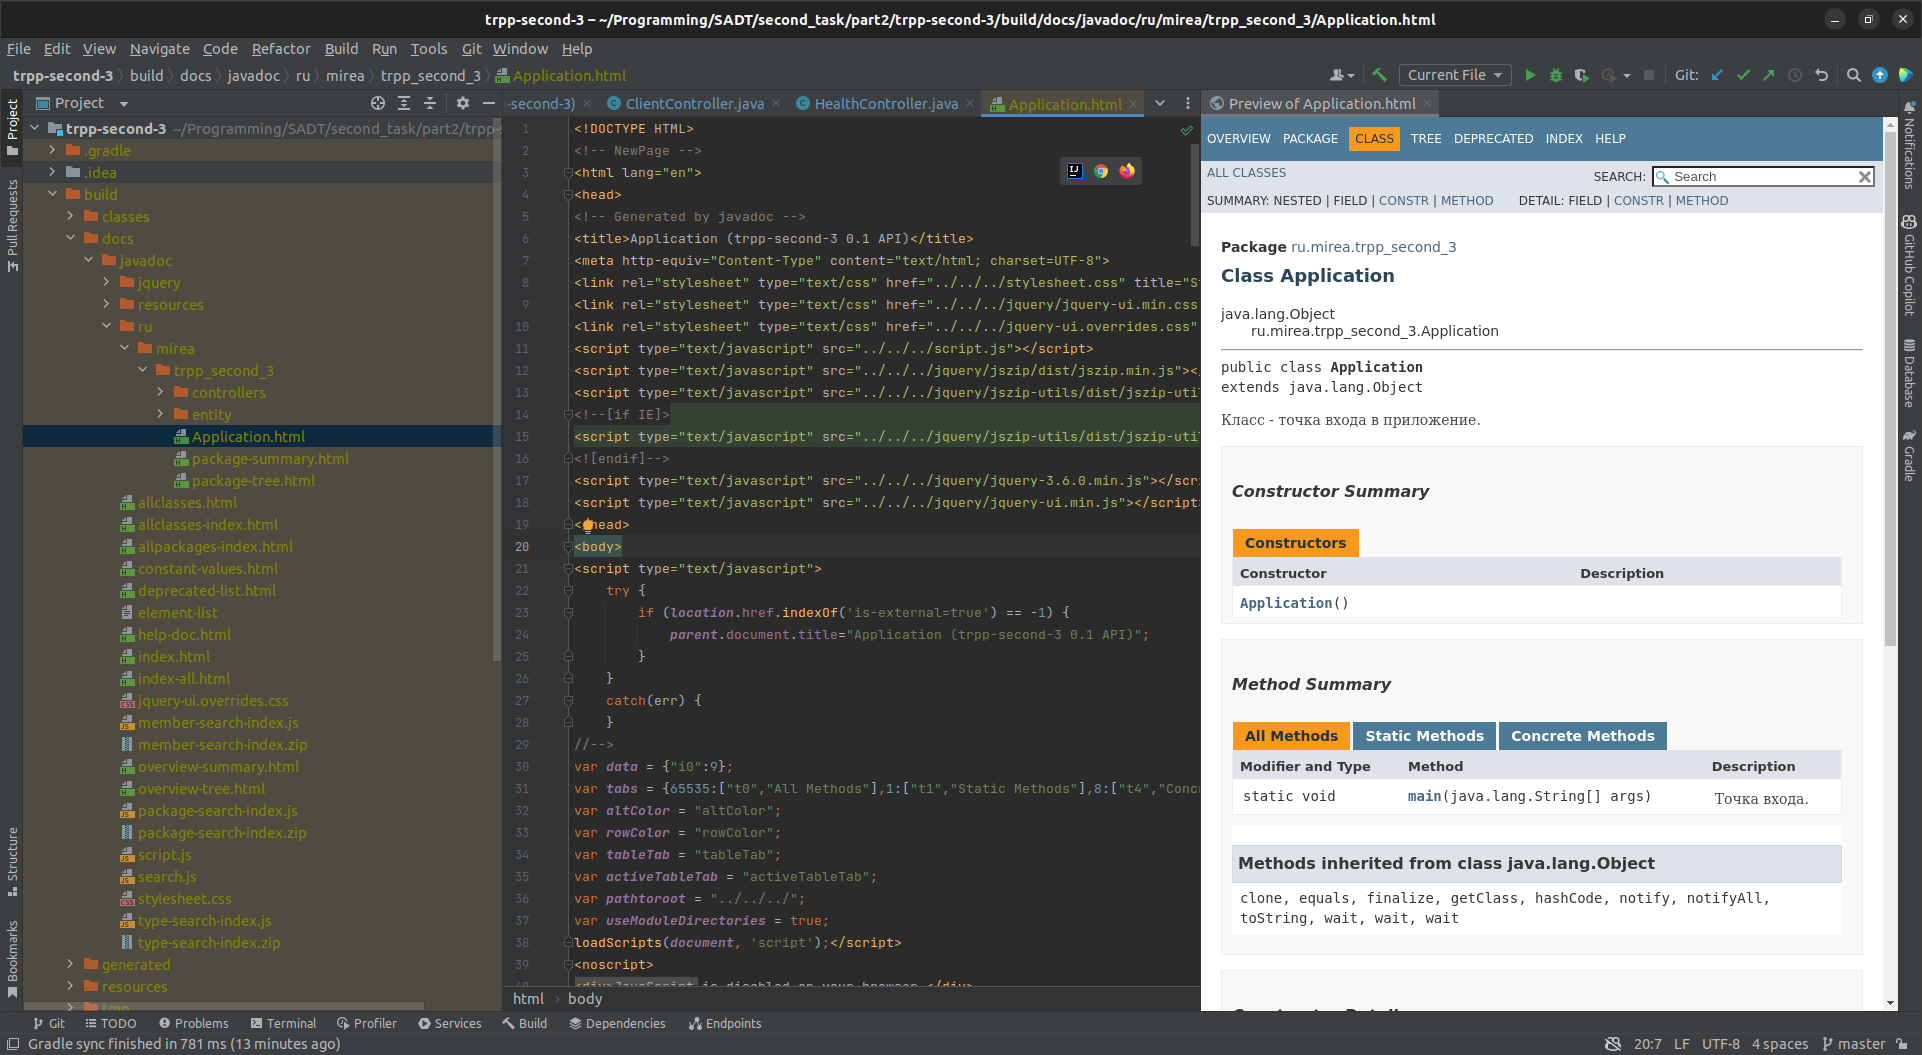
\includegraphics[width=0.8\textwidth]{Screenshot from 2023-03-12 18-27-47.png}
	\caption{Сгенерированая документация}
	\label{fig:gradle:javadoc}
\end{figure}

\section{Сборка jar со всеми зависимостями}
Для генерации jar понадобилась команда \texttt{./gradlew shadowJar},
которая собрает UberJar (архив со всеми зависимостями)
Для запуска приложения используется команда: \texttt{./gradlew run}
(Рисунок~\ref{fig:gradle:run}).

\begin{figure}[h!tp]
	\centering
	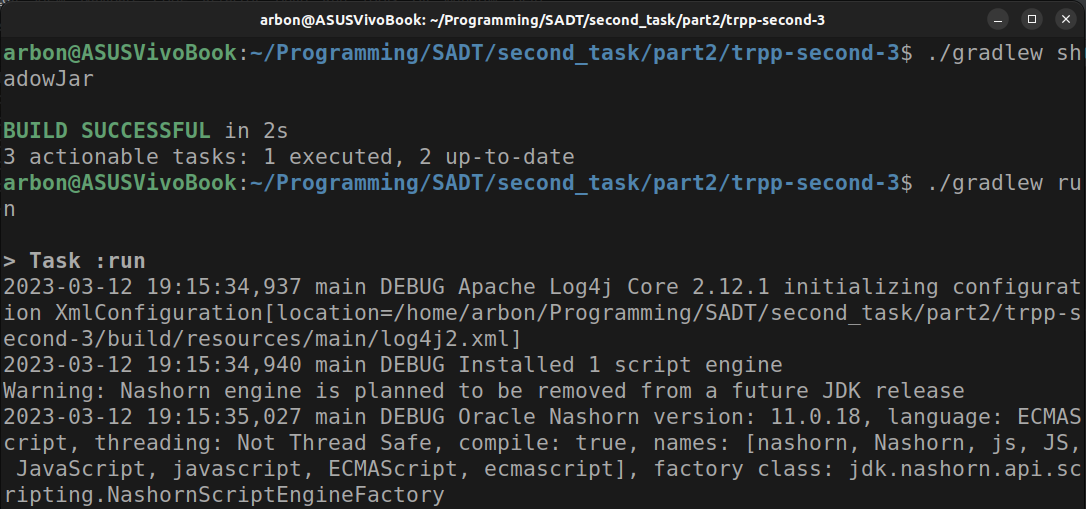
\includegraphics[width=0.8\textwidth]{Screenshot from 2023-03-12 19-16-01.png}
	\caption{Сборка jar и запуск приложения}
	\label{fig:gradle:run}
\end{figure}

\section{Запрос состояния запущенного сервера}
Получить (GET) страницу в Linux можно с помощью команды: \texttt{curl}.
Для этого передадим ей адрес \textit{http://localhost:8080}.
Вывод команды показан на рисунке~\ref{fig:curl}.

\begin{figure}[h!tp]
	\centering
	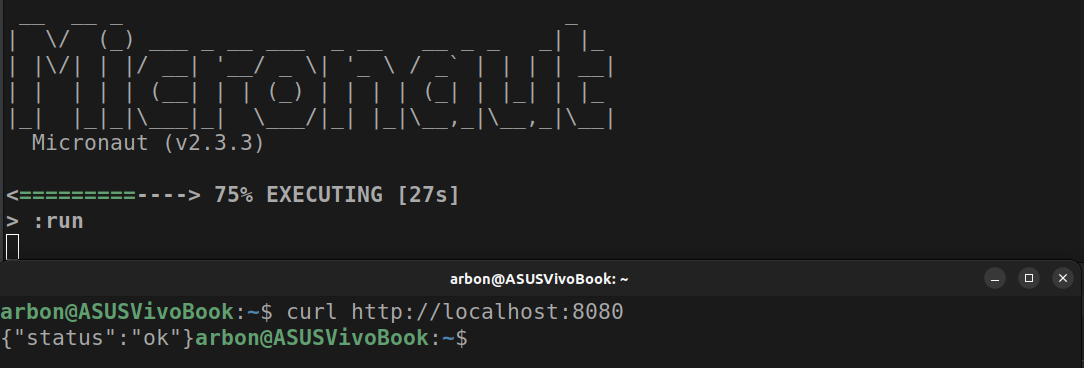
\includegraphics[width=0.8\textwidth]{Screenshot from 2023-03-12 19-51-03.png}
	\caption{GET запрос}
	\label{fig:curl}
\end{figure}

\section{Запрос сущности по идентификатору}
Аналогично примеру выше использовали каманду \texttt{curl},
передав параметром путь \textit{http://localhost:8080/client/874}
(3 последние цифры --- это серийный номер студенческого билета).

\begin{figure}[h!tp]
	\centering
	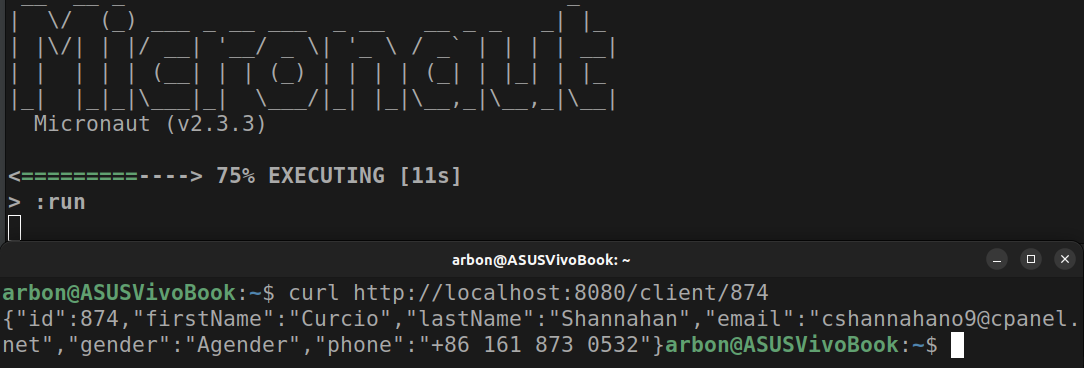
\includegraphics[width=0.8\textwidth]{Screenshot from 2023-03-12 20-08-05.png}
	\caption{GET запрос}
	\label{fig:curl:d}
\end{figure}

\section{В задаче shadowJar добавка к jar-файлу фамилии}
Чтобы добавить к jar-файлу текст нужно изменить файл build.gradle, как
показано на рисунке~\ref{fig:jar:rename}

\begin{figure}[h!tp]
	\centering
	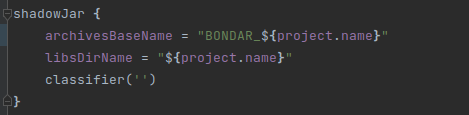
\includegraphics[width=0.8\textwidth]{Screenshot from 2023-03-12 20-32-59.png}
	\caption{Измененный build.gradle}
	\label{fig:jar:rename}
\end{figure}

Теперь после генерации в каталоге build/<имя проекта>/ появиться jar-файл
(Рисунок \ref{fig:jar:file}).

\begin{figure}[h!tp]
	\centering
	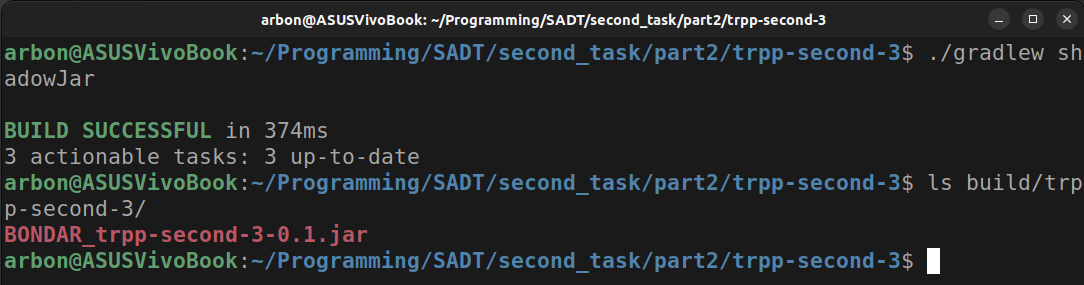
\includegraphics[width=0.8\textwidth]{Screenshot from 2023-03-12 20-32-42.png}
	\caption{Jar-файл}
	\label{fig:jar:file}
\end{figure}

\section{Выполнение задачи checkstyleMain}
Введя команду \texttt{./gradlew checkstyleMain}, она выдает ошибку в
стиле кода и указывает где именно эта ошибка
(Рисунок~\ref{fig:gradle:checkstyleMain}).

\begin{figure}[h!tp]
	\centering
	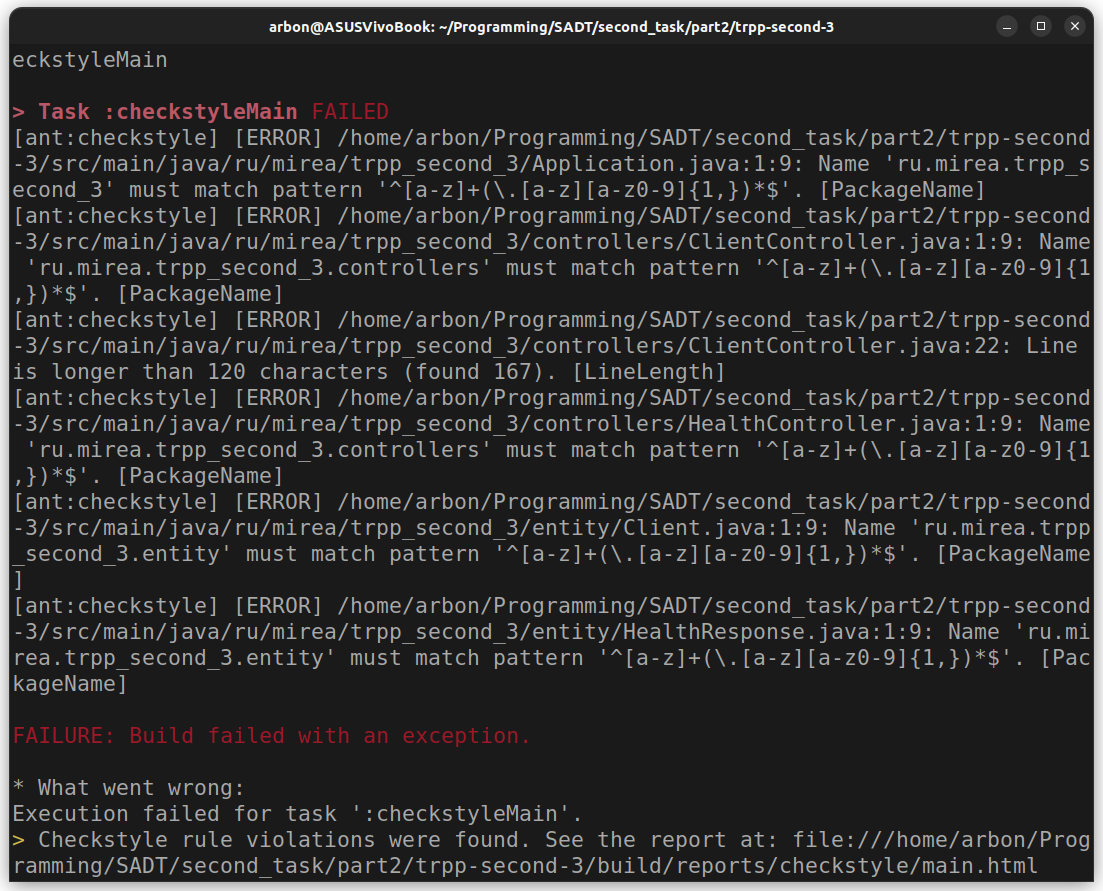
\includegraphics[width=0.9\textwidth]{Screenshot from 2023-03-13 16-57-26.png}
	\caption{Информаци об ошибке в стиле}
	\label{fig:gradle:checkstyleMain}
\end{figure}

А также предлагает открыть сгенерированный отчет. Пример отчета изображен на
рисунках~\ref{fig:gradle:checkstyle:rep:s}\,-\,\ref{fig:gradle:checkstyle:rep:f}.

\begin{figure}[h!tp]
	\centering
	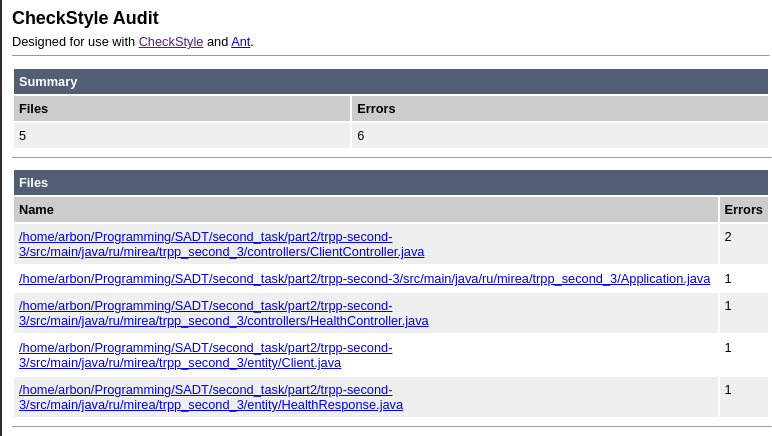
\includegraphics[width=0.9\textwidth]{Screenshot from 2023-03-13 16-47-00.png}
	\caption{Информаци об ошибке в стиле}
	\label{fig:gradle:checkstyle:rep:s}
\end{figure}

\begin{figure}[h!tp]
	\centering
	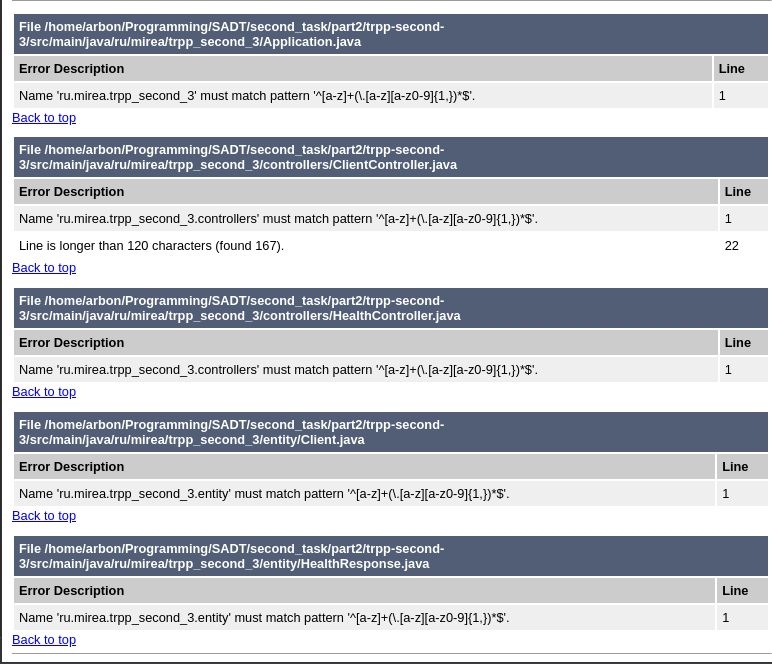
\includegraphics[width=0.9\textwidth]{Screenshot from 2023-03-13 16-48-05.png}
	\caption{Информаци об ошибке в стиле}
	\label{fig:gradle:checkstyle:rep:f}
\end{figure}

\clearpage

\chapter*{Ответы на вопросы}
\addcontentsline{toc}{chapter}{Ответы на вопросы}

\begin{description}
	\item[Что такое система сборки?]
		Система сборки --- это программа, которая собирает другие программы.
		На вход система сборки получает исходный код, а на выход выдаёт
		программу, которую уже можно запустить.
	\item[Что такое gradle?]
		Gradle --- система автоматической сборки, построенная на принципах
		Apache Ant и Apache Maven, но предоставляющая DSL на языках
		Groovy и Kotlin вместо традиционной XML-образной формы представления
		конфигурации проекта.
	\item[Что такое maven?]
		Maven --- инструмент для автоматизации сборки проектов.
		С ним работают в основном Java-разработчики, хотя есть плагины
		для интеграции с C/C++, Ruby, Scala, PHP и другими языками.\par
		Одна из главных особенностей фреймворка --- декларативное описание
		проекта. Это значит, что разработчику не нужно уделять внимание
		каждому аспекту сборки --- все необходимые параметры настроены
		по умолчанию. Изменения нужно вносить лишь в том объёме,
		в котором программист хочет отклониться от стандартных настроек.
	\item[Что делает задача build?]
		Задача \texttt{build} выполнит сборку проекта для продакшена
		(т.е. она запустит \texttt{clean:build}, \texttt{html:build},
		\texttt{css:build}, \texttt{js:build}, \texttt{fonts:build}
		и \texttt{image:build}). Эти задачи поместят
		в каталог "assets/build" результирующие файлы проекта.
	\item[Что такое micronaut?]
		Micronaut --- это фреймворк на JVM для построения легковесных
		модульных приложений.
	\item[Что такое postman?]
		Postman --- это платформа API для создания и использования API.
		Postman упрощает каждый этап жизненного цикла API, а также совместную
		работу, что позволяет быстрее создавать улучшенные API.
\end{description}

\chapter*{Выводы}
\addcontentsline{toc}{chapter}{Выводы}
В данной практической работе научились писать базовые bash скрипты, такие
например как: получение текущего премени, чтение из файл или директории или
получение размеров директории. Также узнали как развертывать и запускать
проект с помощью самостоятельно написаных bash скриптов.\par
Еще в этой работе освоили работу со системой сборки gradle.
Например: разбор ошибок выводящиеся gradle-ом, сборка документации или
создание jar-файла.

